%!TEX program = xelatex
\documentclass{beamer}

\usepackage[spanish]{babel}

\usepackage{graphicx,hyperref,url, materialbeamer}
\usepackage{braket}
%\usepackage{euler}
\usepackage{listings}

\graphicspath{ {./figs/} }
\setbeamercovered{transparent}
\lstdefinestyle{customsql}{
  belowcaptionskip=1\baselineskip,
  tabsize=4,
  breaklines=true,
  xleftmargin=\parindent,
  language=C,
  showstringspaces=false,
  basicstyle=\footnotesize\ttfamily,
  keywordstyle=\bfseries\color{green!40!black},
  commentstyle=\itshape\color{purple!40!black},
  identifierstyle=\color{blue},
  stringstyle=\color{orange},
}
\lstset{escapechar=@,style=customsql}



\usefonttheme{professionalfonts} % using non standard fonts for beamer
%\usefonttheme{serif}

% The title of the presentation:
%  - first a short version which is visible at the bottom of each slide;
%  - second the full title shown on the title slide;
\title[Programación]{Programación}

% Optional: a subtitle to be dispalyed on the title slide
\subtitle{Tronco Común de Ingeniería \\ FCQI}

% The author(s) of the presentation:
%  - again first a short version to be displayed at the bottom;
%  - next the full list of authors, which may include contact information;
\author[Violeta Ocegueda]{Violeta Ocegueda} 
  
%\titlegraphic{\includegraphics[width=\textwidth]{atac-logo}}

% The institute:
%  - to start the name of the university as displayed on the top of each slide
%    this can be adjusted such that you can also create a Dutch version
%  - next the institute information as displayed on the title slide
\institute[UABC]{Profesor-Investigador \\ Facultad de Ciencias Químicas e Ingeniería \\ Universidad Autónoma de Baja California \\ Campus Tijuana}

% Add a date and possibly the name of the event to the slides
%  - again first a short version to be shown at the bottom of each slide
%  - second the full date and event name for the title slide
\date[\today]{\today}

\providecommand{\di}{\mathop{}\!\mathrm{d}}
\providecommand*{\der}[3][]{\frac{d\if?#1?\else^{#1}\fi#2}{d #3\if?#1?\else^{#1}\fi}} 
 \providecommand*{\pder}[3][]{% 
    \frac{\partial\if?#1?\else^{#1}\fi#2}{\partial #3\if?#1?\else^{#1}\fi}% 
  }
\begin{document}

\begin{frame}
  \titlepage
\end{frame}

\begin{frame}
  \frametitle{Contenido}
  \tableofcontents
\end{frame}

%\setlength{\parskip}{\baselineskip} 
\section{Metodología}

\begin{frame}[c] 
\frametitle{}
\centering
\huge \textbf{Metodología para la resolución de problemas}
\end{frame}

\begin{frame}[t]
\frametitle{Metodología para la resolución de problemas}
\begin{block}{\textbf{Problema}}
Un problema se entiende como una proposición que, a partir de ciertas condiciones conocidas, induce a buscar algo desconocido.
\end{block}
El proceso de resolución de un problema con una computadora conduce a la escritura de un programa y a su ejecución en la misma. Aunque el proceso de diseñar programas es -esencialmente- un \textbf{proceso creativo}, se pueden considerar una serie de fases o pasos comunes a seguir.
\end{frame}

\begin{frame}[t]
\frametitle{Metodología para la resolución de problemas}
Las fases de resolución de un problema con computadora son:
\begin{itemize}
    \item Análisis del problema \pause
    \item Diseño del algoritmo \pause
    \item Codificación \pause
    \item Compilación y ejecución \pause
    \item Verificación \pause
    \item Depuración \pause
    \item Mantenimiento \pause
    \item Documentación
\end{itemize}
\end{frame}

\begin{frame}[t]
\frametitle{Análisis del problema}
\begin{itemize}
    \item Es la primera fase de la resolución de un problema con computadora.
    \item Requiere una clara definición de las \textbf{entradas} y \textbf{salidas}.
\end{itemize}
\textbf{Ejercicio:} Describa el proceso de retirar dinero del cajero.
\end{frame}

\begin{frame}[t]
\frametitle{Diseño del algoritmo}
\begin{block}{\textbf{Algoritmo}}
Un algoritmo es un \textcolor{orange}{conjunto de pasos}, procedimientos o acciones que nos permiten alcanzar un resultado o \textcolor{orange}{resolver un problema}.
\end{block}
Un algoritmo se puede concebir como un \textcolor{orange}{diálogo entre una computadora y una persona}, en el que se especifica bajo qué condiciones la computadora debe generar la salida específica.
\end{frame}

\begin{frame}[t]
\frametitle{Características de los algoritmos}
Las características que los algoritmos deben reunir son las siguientes:
\begin{itemize}
    \item \textcolor{blue}{Precisión:} los pasos a seguir en el algoritmo deben ser precisados claramente. \pause
    \item \textcolor{blue}{Determinismo:} dado un conjunto de datos idénticos de entrada, siempre debe arrojar los mismos resultados. \pause
    \item \textcolor{blue}{Finitud:} independientemente de su complejidad, siempre debe ser de longitud finita. 
\end{itemize}
\end{frame}

\begin{frame}[t]
\frametitle{Diagrama de flujo}
Un \textcolor{blue}{diagrama de flujo} representa la \textcolor{orange}{esquematización gráfica} de un algoritmo. Es decir, muestra gráficamente los pasos o procesos a seguir para alcanzar la \textcolor{orange}{solución de un problema}.
\end{frame}

\begin{frame}[t]
\frametitle{Símbolos utilizados en los diagramas de flujo}
\begin{center}
    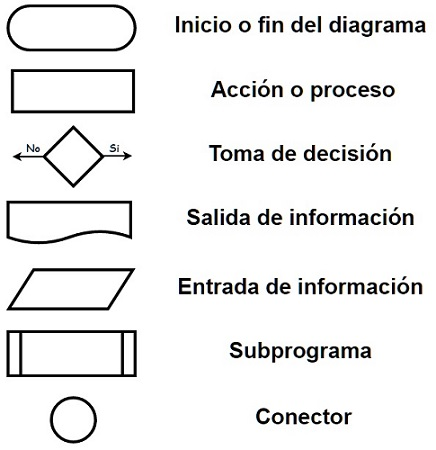
\includegraphics[width=0.57\textwidth]{figs/diagrama_flujo_simbolos}
\end{center}
\end{frame}

\begin{frame}[t]
\frametitle{Codificación}
\textcolor{blue}{Codificación} es la escritura en un lenguaje de programación de la representación del algoritmo desarrollada en etapas anteriores.
\end{frame}

\begin{frame}[t]
\frametitle{Depuración}
La \textcolor{blue}{depuración} es el proceso de encontrar los errores del programa y corregir o eliminar dichos errores.\\
Cuando se ejecuta un programa se pueden producir tres tipos de errores:
\begin{itemize}
    \item \textcolor{blue}{Errores de compilación:} o \textit{errores de sintaxis}, se producen normalmente por un uso incorrecto de las reglas del lenguaje de programación. \pause
    \item \textcolor{blue}{Errores de ejecución:} se producen por instrucciones que la computadora puede comprender pero no ejecutar (división por cero, raíces cuadradas de números negativos). \pause
    \item \textcolor{blue}{Errores lógicos:} se producen en la lógica del programa y la fuente del error suele ser el diseño del algoritmo.
\end{itemize}
\end{frame}


\begin{frame}[t]
\frametitle{Ejercicios}
Realiza el análisis, el algoritmo y el diagrama de flujo de los siguiente problemas:
\begin{itemize}
    \item Calcular la suma de dos números.
    \item Calcular el área de un triángulo.
    \item Calcular la hipotenusa de un triángulo.
    \item Identificar el mayor de dos números.
    \item Identificar el mayor de tres números.
    \item Imprimir los primeros diez números pares.
\end{itemize}
\end{frame}



%\begin{frame}
%\frametitle{Before Tao}
%	\begin{itemize}
% 	\item Facebook was storing the social graph to MySql
%	\begin{itemize}
%		\item  	Quering it from PHP
%		\item  	Storing result in memcache\\
%	\end{itemize}
%	\end{itemize}
%	\begin{center}
%		\includegraphics[width=0.3\textwidth]{figs/php-logo.eps}\quad
%		\includegraphics[width=0.3\textwidth]{figs/mysql.png}
%	\end{center}
% 	Over time Fb deprecated direct access to MySQL in favor of a graph (associations, nodes) abstraction
%\end{frame}




%!TEX root = P_Manual.tex
\setlength{\parskip}{\baselineskip} 
\section{Lenguaje}

% ----------------------- Slide 01-------------------------------- %
\begin{frame}[c] 
\frametitle{}
\centering
\huge \textbf{Introducción al lenguaje de programación}
\end{frame}


% --------------------------- Slide 02 ---------------------------------- %
\begin{frame}[t, fragile]{Estructura básica de un programa}
%	\frametitle{Estructura básica de un programa}
	\begin{lstlisting}
/* Inclusion de librerias */

void main() /* cabecera de funcion */
{ /* inicio de la funcion main */

... /* Sentencias */

} /* fin de la funcion main */
\end{lstlisting}
\end{frame}


% ------------------------- Slide 03 --------------------------------- %
\begin{frame}[fragile]{Estructura básica de un programa para la clase}
%	\frametitle{Estructura básica de un programa para la clase}
	\begin{lstlisting}
/* Inclusion de librerias */

void main() /* cabecera de funcion */
{ /* inicio de la funcion main */

/* Declaracion de variables */

/* Entrada de datos */

/* Procesamiento */

/* Impresion de resultados */

} /* fin de la funcion main */
\end{lstlisting}
\end{frame}


% -------------------------- Slide 04 ---------------------------------- %
\begin{frame}[fragile, t]{Zonas de memoria}
%	\frametitle{Zonas de memoria}
	\textbf{Variables}\\
	\footnotesize
	\begin{itemize}
		\item Son objetos que pueden cambiar su valor durante la ejecución de un programa.
		\item En C una \textit{variable} es una posición en memoria con nombre donde se almacena un valor de un cierto tipo de dato.
	\end{itemize}
	\vspace{-2mm}
	La \textit{declaración} de una variable es una sentencia que proporciona información de la variable al compilador C. Su sintaxis es:
	\begin{lstlisting}
<tipo_variable> <nombre_variable> = <valor_inicial>;
\end{lstlisting}
	\vspace{-4mm}
	Donde:
	\vspace{-4mm}
	\begin{itemize}
		\item \textit{tipo\_variable} es el nombre de un tipo de dato conocido por C.
		\item \textit{nombre\_variable} es un identificador (nombre) válido en C.
		\item \textit{valor\_inicial} es el valor de inicialización de la variable.
	\end{itemize}
\end{frame}

% --------------------------- Slide 05 --------------------------------- %
\begin{frame}[t, fragile]{Zonas de memoria}
	%\frametitle{Zonas de memoria}
	\textbf{Tipos de datos}\\
	\footnotesize
	Los tipos de datos básicos son:
	\begin{itemize}
		\item enteros
		\item flotantes
		\item caracteres
	\end{itemize}
	\textbf{Constantes}\\
	Las \textit{constantes} son datos que no cambian durante la ejecución de un programa.
	\begin{lstlisting}
#define NUEVALINEA \n 
#define PI 3.141592 
#define VALOR 54
\end{lstlisting}
\end{frame}


% --------------------------- Slide 06 --------------------------------- %
\begin{frame}[t]{Operadores}
\textbf{Operadores de asignación y expresión}\\
\begin{center}
	\begin{tabular}{ccc}
		\toprule
		\textbf{Operador} & \textbf{Expresión} & \textbf{Explicación} \\
		\midrule
		+= & c += 7 & c = c + 7 \\ \hline
		-= & d -= 4 & d = d - 4 \\ \hline
		*= & e *= 5 & e = e * 5 \\ \hline
		/= & f/= 3 & f = f / 3 \\ \hline
		\hspace{1mm} \%= & g \%= 9 & g = g \% 9 \\
		\bottomrule
	\end{tabular}
\end{center}
\end{frame}

% --------------------------- Slide 07 --------------------------------- %
\begin{frame}[t]{Operadores}
\textbf{Operadores aritméticos}\\
\vspace{5mm}
\small
\begin{center}
	\begin{tabular}{cccc}
		\toprule
		\textbf{Operador} & \textbf{Operación} & \textbf{Expresión algebraica} & \textbf{Expresión en C}\\
		\midrule
		+ & Suma & f + 7 & f + 7 \\ \hline
		- & Resta & p - c & p - c\\ \hline
		* & Multiplicación & bm & b * m\\ \hline
		/ & División & $\frac{x}{y}$ ó $\sfrac{x}{y}$ & x / y \\ \hline
	\end{tabular}
\end{center}
\end{frame}

% --------------------------- Slide 08 --------------------------------- %
\begin{frame}[t]{Operadores}
\textbf{Operadores de relación}\\ \vspace{5mm}
\begin{center}
\begin{tabular}{ccl}
	\toprule
	\textbf{Operador} & \textbf{Ejemplo} & \textbf{Significado}\\
	\midrule
	== & x == y & x es igual que y \\ \hline
	!= & x != y & x es diferente de y \\ \hline
	> & x > y & x es mayor que y \\ \hline
	< & x < y & x es menor que y \\ \hline
	>= & x >= y & x es mayor o igual que y \\ \hline
	<= & x <= y & x es menos o igual que y \\ 
	\bottomrule
\end{tabular}
\end{center}
\end{frame}

% --------------------------- Slide 09 --------------------------------- %
\begin{frame}[t]{Operadores}
\textbf{Operadores lógicos: AND lógico}\\ \vspace{3mm}
\small
\begin{center}
%\caption{Tabla de verdad para el operador \textit{\&\&} (AND l\'ogico).}
\begin{tabular}{llc}
	\toprule
	\textbf{expresión} & \textbf{expresión2} & \textbf{expresión1 \&\& expresión2}\\
	\midrule \hline
	0 & 0 & 0 \\
	0 & diferente de cero & 0\\
	diferente de cero & 0 & 0\\
	diferente de cero & diferente de cero & 1\\ \hline
	\bottomrule
\end{tabular}
\end{center}
\end{frame}

% --------------------------- Slide 10 ------------------------------ %
\begin{frame}[t]{Operadores}
\textbf{Operadores lógicos: OR lógico}\\ \vspace{5mm}
\centering
%\caption{Tabla de verdad para el operador \textit{| |} (OR l\'ogico).}
\begin{tabular}{llc}
	\toprule
	\textbf{expresión1} & \textbf{expresión2} & \textbf{expresión1 $| |$ expresión2}\\
	\midrule \hline
	0 & 0 & 0 \\
	0 & diferente de cero & 1\\
	diferente de cero & 0 & 1\\
	diferente de cero & diferente de cero & 1\\ \hline
	\bottomrule
\end{tabular}
\end{frame}

% --------------------------- Slide 11 --------------------------------- %
\begin{frame}[t]
\frametitle{Operadores}
\textbf{Operadores lógicos: NOT lógico}\\ \vspace{5mm}
\centering
%\caption{Tabla de verdad para el operador \textbf{!} (negaci\'on l\'ogico).}
\begin{tabular}{lc}
\toprule
\textbf{expresión} & \textbf{!expresión}\\
\midrule \hline
0 & 1 \\
diferente de cero & 0\\
\bottomrule
\end{tabular}
\end{frame}

% --------------------------- Slide 12 --------------------------------- %
\begin{frame}[t]{Operadores}
\textbf{Operadores de incremento y decremento}\\ \vspace{5mm}
\footnotesize
\begin{center}
%\caption{Operadores de incremento y decremento}
\begin{tabular}{ccp{7.5cm}}
	\toprule
	\textbf{Operador} & \textbf{Ejemplo} & \textbf{Explicación}\\
	\midrule
	++&++a& Incrementar a en 1 y después utiliza el nuevo valor de a en la expresión en la que reside.\\
	++ & a++ & Utiliza el valor actual de a en la expresión en la que reside, y después la incrementa en 1.\\
	$--$ & $--$b & Decrementar b en 1 y después utiliza el nuevo valor de b en la expresión en la que reside.\\
	$--$ & b$--$ & Utiliza el valor actual de b en la expresión en la que reside, y después decrementa b en 1.\\
	\bottomrule
\end{tabular}
\end{center}
\end{frame}


% --------------------------- Slide 13 --------------------------------- %
\begin{frame}[t]{Operadores}
\textbf{Jerarquía de operadores}\\ \vspace{5mm}
\scriptsize
%\begin{table}[h]
\centering
%\caption{Jerarqu\'ia de operadores}
\begin{tabular}{ccll}
	\toprule
	\textbf{Jerarqu\'ia} & \textbf{Operadores} & \textbf{Asociatividad} & \textbf{Tipo}\\ 
	\midrule 
	Mayor & $++$ $--$ $+$ $-$ $!$ & derecha a izquierda & unario\\ \cline{2-4}
	| & * / \% & izquierda a derecha & multiplicativo\\ \cline{2-4}
	| & + $-$ & izquierda a derecha & aditivo\\ \cline{2-4}
	| & $<$ $<=$ $>$ $>=$ & izquierda a derecha & de relaci\'on \\ \cline{2-4}
	| & == != & izquierda a derecha & de relación\\ \cline{2-4}
	| & \&\& & izquierda a derecha & AND lógico\\ \cline{2-4}
	| & $| |$ & izquierda a derecha & OR lógico \\ \cline{2-4}
	Menor & $=$, $+=$, $-=$, $*=$, $/=$, $\%=$ & derecha a izquierda & de asignación \\ 
	\bottomrule
\end{tabular}
%\end{table}
\end{frame}


% --------------------------- Slide 14 --------------------------------- %
\begin{frame}{Instrucción de salida}
La instrucción de salida utilizada en C se denomina \textbf{printf}. Su sintaxis es:\\
\vspace{5mm}

{\small \textit{printf( ``texto a imprimir'' );}\\
\textit{printf( ``texto a imprimir \%formato\_de\_impresión'',variable\_a\_imprimir );}}
\end{frame}


% --------------------------- Slide 15 --------------------------------- %
\begin{frame}[t]
\frametitle{Formato de salida con printf}
\textbf{Especificadores de conversión entera para \textit{printf}}\\ \vspace{5mm}
\scriptsize
%\begin{table}[h]
\begin{center}
%\caption{Especificadores de conversi\'on entera para \textit{printf}}
\begin{tabular}{lp{7.5cm}}
	\toprule
	\textbf{Especificador} & \textbf{Descripción}\\
	\midrule
	\textbf{\%d} & Despliega un entero decimal con signo.\\ 
	\textbf{\%i} & Despliega un entero decimal con signo. [Nota: los especificadores i y d son diferentes cuando se utilizan con \textbf{scanf}.]\\ 
	\textbf{\%o} & Despliega un entero octal sin signo.\\
	\textbf{\%u} & Despliega un entero decimal sin signo. \\
	\textbf{\%x} ó \textbf{\%X} & Despliega un entero hexadecimal sin signo. \textbf{X} provoca que se desplieguen los dígitos de \textbf{0} a \textbf{9} y las letras de \textbf{A} a \textbf{F}, y \textbf{x} provoca que se desplieguen los dígitos de \textbf{0} a \textbf{9} y las letras de \textbf{a} a \textbf{f}.\\ 
	\textbf{h} ó \textbf{l} (letra l) & Se coloca antes de cualquier especificador de conversión entera para indicar que se despliega un entero corto o largo, respectivamente. Las letras \textbf{h} y \textbf{l} son llamadas con más precisión \textit{modificadores de longitud}.\\
	\bottomrule
\end{tabular}
%\end{table}
\end{center}
\end{frame}
% --------------------------- Slide 16 --------------------------------- %
\begin{frame}[t]{Formato de salida con printf}
\textbf{Especificadores de conversi\'on de punto flotante para \textit{printf}}\\ \vspace{5mm}
\scriptsize
\centering
%\caption{Especificadores de conversi\'on de punto flotante para \textit{printf}}
\begin{tabular}{lp{7.5cm}}
	\toprule
	\textbf{Especificador} & \textbf{Descripción}\\
	\midrule 
	\textbf{\%e} \'o \textbf{\%E} & Despliega un valor de punto flotante con notaci\'on exponencial.\\
	\textbf{\%f} & Despliega un valor de punto flotante con notaci\'on de punto fijo.\\
	\textbf{\%g} \'o \textbf{\%G} & Despliega un valor de punto flotante con el formato de punto flotante \textbf{f}, o con el formato exponencial \textbf{e} (o \textbf{E}) basado en la magnitud del valor. \\
	\textbf{L} & Se coloca antes del especificador de conversión para indicar que se desplegar\'a un valor de punto flotante \textbf{long double}\\ 
	\bottomrule
\end{tabular}
\end{frame}

% --------------------------- Slide 17 --------------------------------- %
\begin{frame}[t]{Formato de salida con printf}
\textbf{Especificadores de conversión de caracteres y cadenas para \textit{printf}}\\ \vspace{5mm}
%\scriptsize
\centering
%\caption{Especificadores de conversi\'on de caracteres y cadenas para \textit{printf}}
\begin{tabular}{lp{7.5cm}}
	\toprule
	\textbf{Especificador} & \textbf{Descripci\'on}\\
	\midrule
	\textbf{\%c} & Despliega caracteres individuales.\\
	\textbf{\%s} & Despliega cadenas de caracteres. \\
	\bottomrule
\end{tabular}
\end{frame}

% --------------------------- Slide 18 --------------------------------- %
\begin{frame}[t]{Formato de salida con printf}
\textbf{Otros especificadores de conversi\'on para \textit{printf}}\\ \vspace{5mm}
\scriptsize
\begin{center}
%\caption{Otros especificadores de conversi\'on para \textit{printf}}
\begin{tabular}{lp{7.5cm}}
	\toprule
	\textbf{Especificador} & \textbf{Descripción}\\
	\midrule
	\textbf{\%p} & Despliega un valor apuntador de manera definida por la implementación.\\ 
	\textbf{\%n} & Almacena el número de caracteres ya desplegados en la instrucci\'on \textbf{printf} actual. Proporciona un apuntador a un entero como el argumento correspondiente. No despliega valor alguno.\\ 
	\textbf{\%\%} & Despliega el caracter de porcentaje.\\
	\bottomrule
\end{tabular}
\end{center}
\end{frame}

% --------------------------- Slide 19 --------------------------------- %
\begin{frame}[t]{Secuencias de escape}
\small
\begin{center}
\begin{tabular}{p{3.5cm}p{6.5cm}}
	\toprule
	\textbf{Secuencia de escape} & \textbf{Descripción}\\
	\midrule
	\textbackslash a (alerta o campana) & Provoca una alerta sonora (campana) o una alerta visual.\\
	\textbackslash \textbackslash (diagonal invertida) & Despliega el caracter de diagonal invertida (\textbackslash).\\
	\textbackslash ' (comilla sencilla) & Despliega el caracter de comilla sencilla (').
	\\
	\textbackslash '' (comilla doble) & Despliega el caracter de comilla doble (''). \\ 
	\textbackslash ? (interrogación) & Despliega el caracter de interrogación (?).\\
	\textbackslash n (nueva línea) & Mueve el cursor al inicio de la siguiente línea.\\
	\bottomrule
\end{tabular}
\end{center}
\end{frame}

% --------------------------- Slide 20 --------------------------------- %
\begin{frame}[t]{Secuencias de escape (Continuación)}
\vspace{-4mm}
\small
\begin{center}
	\begin{tabular}{p{4cm}p{6cm}}
		\toprule
		\textbf{Secuencia de escape} & \textbf{Descripción}\\
		\midrule 
		\textbackslash t (tabulador horizontal) & Mueve el cursor a la siguiente posición del tabulador.\\
		\textbackslash b (retroceso) & Mueve el cursor una posición hacia atrás en la línea actual.\\
		\textbackslash f (nueva página o avance de página) & Mueve el cursor al inicio de la siguiente página l\'ogica.\\
		\textbackslash r (retorno de carro) & Mueve el cursor al principio de la línea actual.\\
		\textbackslash v (tabulador vertical) & Mueve el cursor a la siguiente posición del tabulador vertical.\\
		\bottomrule
	\end{tabular}
\end{center}
\end{frame}

% --------------------------- Slide 21 --------------------------------- %
\begin{frame}{Banderas de la cadena de control de formato}
\small
%\begin{table}[h]
\centering
%\caption{Banderas de la cadena de control de formato}
\begin{tabular}{lp{6cm}}
	\toprule
	\textbf{Bandera} & \textbf{Descripción}\\
	\midrule 
	\textbackslash$-$ (signo menos) & Justifica la salida a la izquierda dentro del campo especificado.\\ 
	\hline
	\textbackslash+ (signo más) & Despliega el signo más que precede a los valores positivos, y un signo menos que precede a los valores negativos.\\
	\hline
	\textit{espacio} & Imprime un espacio antes de un valor positivo no impreso con la bandera +.\\
	\bottomrule
\end{tabular}
%\end{table}
\end{frame}

% --------------------------- Slide 22 --------------------------------- %
\begin{frame}[t]{Instrucción de entrada}
La instrucción de entrada utilizada en C se denomina \textbf{scanf}. Su sintaxis es:\\
\textit{scanf( ``especificador\_de\_conversión'',\&nombre\_variable );}\\
Donde:
%----------LIST----------
\begin{itemize}
	\item \textbf{especificador\_de\_conversión} describe el formato de los datos de entrada.
	\item \textbf{\&} asigna los datos, en el formato especificado, a la variable especificada.
	\item \textbf{nombre\_variable} variable a la cual se le asigna los datos de entrada.
\end{itemize}
\end{frame}

% --------------------------- Slide 23 --------------------------------- %
\begin{frame}[t]{Formato de entrada con scanf}
\textbf{Especificadores de conversi\'on de enteros para \textit{scanf}}
\vspace{-2mm}
\small
\begin{center}
%\caption{Especificadores de conversi\'on de enteros para \textit{scanf}.}
\begin{tabular}{lp{6cm}}
	\toprule
	\textbf{Especificador} & \textbf{Descripci\'on}\\
	\midrule
	\%d & Lee un entero decimal con signo (el signo es opcional). El argumento correspondiente es un apuntador a un entero. \\
	\%i & Lee un entero decimal, octal, o hexadecimal con signo (opcional). El argumento correspondiente es un apuntador a un entero.\\
	\%o & Lee un entero octal. El argumento corespondiente es un apuntador a un entero sin signo.\\
	\bottomrule
\end{tabular}
\end{center}
\end{frame}

% --------------------------- Slide 24 --------------------------------- %
\begin{frame}[t]{Formato de entrada con scanf (Continuación)}
\textbf{Especificadores de conversi\'on de enteros para \textit{scanf}}
\vspace{-2mm}
\small
\begin{center}
	%\caption{Especificadores de conversi\'on de enteros para \textit{scanf}.}
	\begin{tabular}{lp{6cm}}
		\toprule
		\textbf{Especificador} & \textbf{Descripci\'on}\\
		\midrule
		\%u & Lee un entero decimal sin signo. El argumento correspondiente es un apuntador a un entero sin signo.\\
		\%x o \%X & Lee un entero hexadecimal. El argumento correspondiente es un apuntador a un entero sin signo.\\
		h \'o l & Se coloca antes de cualquier especificador de conversi\'on, para indicar que se introducir\'a un entero corto o largo, respectivamente.\\
		\bottomrule
	\end{tabular}
\end{center}
\end{frame}

% --------------------------- Slide 25 --------------------------------- %
\begin{frame}[t]
\frametitle{Formato de entrada con scanf}
\textbf{Especificadores de conversión de números de punto flotante para \textit{scanf}}\vspace{5mm}
\scriptsize
%\begin{table}[h]
\centering
%\caption{Especificadores de conversi\'on de n\'umeros de punto flotante para \textit{scanf}.}
\begin{tabular}{lp{6cm}}
	\toprule
	\textbf{Especificador} & \textbf{Descripci\'on}\\
	\midrule
	\%e, \%E, \%f, \%g \'o \%G & Lee un valor de punto flotante. El argumento correspondiente es un apuntador a un valor de punto flotante.\\
	l \'o L & Se coloca antes de cualquier especificador de conversión para indicar que se introducir\'a un valor \textbf{double} o \textbf{long double}. El argumento correspondiente es un apuntador a una varible \textbf{double} o \textbf{long double}.\\ 
	\bottomrule
\end{tabular}
\end{frame}

% --------------------------- Slide 26 --------------------------------- %
\begin{frame}[t]
\frametitle{Formato de entrada con scanf}
\textbf{Especificadores de conversión de cadenas y caracteres para \textit{scanf}}\vspace{5mm}\\
\scriptsize
\centering
\begin{tabular}{lp{6cm}}
	\toprule
	\textbf{Especificador} & \textbf{Descripción}\\
	\midrule
	\%c & Lee un caracter. El argumento correspondiente es un apuntador a \textbf{char}; no agrega el caracter nulo ('\textbackslash0').\\
	\%s & Lee una cadena. El argumento correspondiente es un apuntador a un arreglo de tipo \textbf{char} que sea lo suficientemente grande para almacenar la cadena y el caracter nulo ('\textbackslash0'), el cual se agrega automáticamente. \\
	\bottomrule
\end{tabular}
\end{frame}
%\input{introduction}
%\input{datamodel}
%\input{architechture}
%\input{implementation}
%\input{consistency}
%\input{workload}

\setbeamercolor{background canvas}{bg=matblue}
\setbeamercolor{normal text}{fg=white}
\begin{frame}[plain, b]
	\centering
	\huge \textcolor{white}{Gracias}
	\normalsize
	\vspace*{\fill}
	
	\begin{beamercolorbox}[wd=\paperwidth]{section in head/foot}
 		\centering
		UABC - FCQI- TCI - Programación
		\vskip10pt
	\end{beamercolorbox}
 \end{frame}

\end{document}
